\documentclass[]{article}
\usepackage{lmodern}
\usepackage{amssymb,amsmath}
\usepackage{ifxetex,ifluatex}
\usepackage{fixltx2e} % provides \textsubscript
\ifnum 0\ifxetex 1\fi\ifluatex 1\fi=0 % if pdftex
  \usepackage[T1]{fontenc}
  \usepackage[utf8]{inputenc}
\else % if luatex or xelatex
  \ifxetex
    \usepackage{mathspec}
  \else
    \usepackage{fontspec}
  \fi
  \defaultfontfeatures{Ligatures=TeX,Scale=MatchLowercase}
\fi
% use upquote if available, for straight quotes in verbatim environments
\IfFileExists{upquote.sty}{\usepackage{upquote}}{}
% use microtype if available
\IfFileExists{microtype.sty}{%
\usepackage{microtype}
\UseMicrotypeSet[protrusion]{basicmath} % disable protrusion for tt fonts
}{}
\usepackage[margin=1in]{geometry}
\usepackage{hyperref}
\hypersetup{unicode=true,
            pdftitle={Analysis of Teaching Evaluations},
            pdfauthor={Dave Bridges},
            pdfborder={0 0 0},
            breaklinks=true}
\urlstyle{same}  % don't use monospace font for urls
\usepackage{color}
\usepackage{fancyvrb}
\newcommand{\VerbBar}{|}
\newcommand{\VERB}{\Verb[commandchars=\\\{\}]}
\DefineVerbatimEnvironment{Highlighting}{Verbatim}{commandchars=\\\{\}}
% Add ',fontsize=\small' for more characters per line
\usepackage{framed}
\definecolor{shadecolor}{RGB}{248,248,248}
\newenvironment{Shaded}{\begin{snugshade}}{\end{snugshade}}
\newcommand{\KeywordTok}[1]{\textcolor[rgb]{0.13,0.29,0.53}{\textbf{#1}}}
\newcommand{\DataTypeTok}[1]{\textcolor[rgb]{0.13,0.29,0.53}{#1}}
\newcommand{\DecValTok}[1]{\textcolor[rgb]{0.00,0.00,0.81}{#1}}
\newcommand{\BaseNTok}[1]{\textcolor[rgb]{0.00,0.00,0.81}{#1}}
\newcommand{\FloatTok}[1]{\textcolor[rgb]{0.00,0.00,0.81}{#1}}
\newcommand{\ConstantTok}[1]{\textcolor[rgb]{0.00,0.00,0.00}{#1}}
\newcommand{\CharTok}[1]{\textcolor[rgb]{0.31,0.60,0.02}{#1}}
\newcommand{\SpecialCharTok}[1]{\textcolor[rgb]{0.00,0.00,0.00}{#1}}
\newcommand{\StringTok}[1]{\textcolor[rgb]{0.31,0.60,0.02}{#1}}
\newcommand{\VerbatimStringTok}[1]{\textcolor[rgb]{0.31,0.60,0.02}{#1}}
\newcommand{\SpecialStringTok}[1]{\textcolor[rgb]{0.31,0.60,0.02}{#1}}
\newcommand{\ImportTok}[1]{#1}
\newcommand{\CommentTok}[1]{\textcolor[rgb]{0.56,0.35,0.01}{\textit{#1}}}
\newcommand{\DocumentationTok}[1]{\textcolor[rgb]{0.56,0.35,0.01}{\textbf{\textit{#1}}}}
\newcommand{\AnnotationTok}[1]{\textcolor[rgb]{0.56,0.35,0.01}{\textbf{\textit{#1}}}}
\newcommand{\CommentVarTok}[1]{\textcolor[rgb]{0.56,0.35,0.01}{\textbf{\textit{#1}}}}
\newcommand{\OtherTok}[1]{\textcolor[rgb]{0.56,0.35,0.01}{#1}}
\newcommand{\FunctionTok}[1]{\textcolor[rgb]{0.00,0.00,0.00}{#1}}
\newcommand{\VariableTok}[1]{\textcolor[rgb]{0.00,0.00,0.00}{#1}}
\newcommand{\ControlFlowTok}[1]{\textcolor[rgb]{0.13,0.29,0.53}{\textbf{#1}}}
\newcommand{\OperatorTok}[1]{\textcolor[rgb]{0.81,0.36,0.00}{\textbf{#1}}}
\newcommand{\BuiltInTok}[1]{#1}
\newcommand{\ExtensionTok}[1]{#1}
\newcommand{\PreprocessorTok}[1]{\textcolor[rgb]{0.56,0.35,0.01}{\textit{#1}}}
\newcommand{\AttributeTok}[1]{\textcolor[rgb]{0.77,0.63,0.00}{#1}}
\newcommand{\RegionMarkerTok}[1]{#1}
\newcommand{\InformationTok}[1]{\textcolor[rgb]{0.56,0.35,0.01}{\textbf{\textit{#1}}}}
\newcommand{\WarningTok}[1]{\textcolor[rgb]{0.56,0.35,0.01}{\textbf{\textit{#1}}}}
\newcommand{\AlertTok}[1]{\textcolor[rgb]{0.94,0.16,0.16}{#1}}
\newcommand{\ErrorTok}[1]{\textcolor[rgb]{0.64,0.00,0.00}{\textbf{#1}}}
\newcommand{\NormalTok}[1]{#1}
\usepackage{longtable,booktabs}
\usepackage{graphicx,grffile}
\makeatletter
\def\maxwidth{\ifdim\Gin@nat@width>\linewidth\linewidth\else\Gin@nat@width\fi}
\def\maxheight{\ifdim\Gin@nat@height>\textheight\textheight\else\Gin@nat@height\fi}
\makeatother
% Scale images if necessary, so that they will not overflow the page
% margins by default, and it is still possible to overwrite the defaults
% using explicit options in \includegraphics[width, height, ...]{}
\setkeys{Gin}{width=\maxwidth,height=\maxheight,keepaspectratio}
\IfFileExists{parskip.sty}{%
\usepackage{parskip}
}{% else
\setlength{\parindent}{0pt}
\setlength{\parskip}{6pt plus 2pt minus 1pt}
}
\setlength{\emergencystretch}{3em}  % prevent overfull lines
\providecommand{\tightlist}{%
  \setlength{\itemsep}{0pt}\setlength{\parskip}{0pt}}
\setcounter{secnumdepth}{0}
% Redefines (sub)paragraphs to behave more like sections
\ifx\paragraph\undefined\else
\let\oldparagraph\paragraph
\renewcommand{\paragraph}[1]{\oldparagraph{#1}\mbox{}}
\fi
\ifx\subparagraph\undefined\else
\let\oldsubparagraph\subparagraph
\renewcommand{\subparagraph}[1]{\oldsubparagraph{#1}\mbox{}}
\fi

%%% Use protect on footnotes to avoid problems with footnotes in titles
\let\rmarkdownfootnote\footnote%
\def\footnote{\protect\rmarkdownfootnote}

%%% Change title format to be more compact
\usepackage{titling}

% Create subtitle command for use in maketitle
\newcommand{\subtitle}[1]{
  \posttitle{
    \begin{center}\large#1\end{center}
    }
}

\setlength{\droptitle}{-2em}
  \title{Analysis of Teaching Evaluations}
  \pretitle{\vspace{\droptitle}\centering\huge}
  \posttitle{\par}
  \author{Dave Bridges}
  \preauthor{\centering\large\emph}
  \postauthor{\par}
  \predate{\centering\large\emph}
  \postdate{\par}
  \date{1/28/2018}


\begin{document}
\maketitle

{
\setcounter{tocdepth}{2}
\tableofcontents
}
\subsection{Data Import}\label{data-import}

Copied evaluation table, added quotes around the questions and imported
into excel. Converted this to a csv file for import. Did this for both
2016 and 2017 teaching evaluations, downloaded from wolverine access.

\begin{Shaded}
\begin{Highlighting}[]
\KeywordTok{library}\NormalTok{(readr)}
\KeywordTok{library}\NormalTok{(dplyr)}
\NormalTok{data.}\FloatTok{2016.}\NormalTok{datafile <-}\StringTok{ '2016 Evaluations.csv'}
\NormalTok{data.}\FloatTok{2017.}\NormalTok{datafile <-}\StringTok{ '2017 Evaluations.csv'}

\NormalTok{input_col_types <-}\StringTok{ }\KeywordTok{cols}\NormalTok{(}
  \DataTypeTok{Number =} \KeywordTok{col_factor}\NormalTok{(}\DataTypeTok{levels=}\OtherTok{NULL}\NormalTok{),}
  \DataTypeTok{Question =} \KeywordTok{col_factor}\NormalTok{(}\DataTypeTok{levels=}\OtherTok{NULL}\NormalTok{))}

\NormalTok{data.}\DecValTok{2016}\NormalTok{ <-}\StringTok{ }\KeywordTok{read_csv}\NormalTok{(data.}\FloatTok{2016.}\NormalTok{datafile, }\DataTypeTok{col_types=}\NormalTok{input_col_types) }\OperatorTok\StringTok{ }\KeywordTok{mutate}\NormalTok{(}\DataTypeTok{Year=}\StringTok{"2016"}\NormalTok{)}
\NormalTok{data.}\DecValTok{2017}\NormalTok{ <-}\StringTok{ }\KeywordTok{read_csv}\NormalTok{(data.}\FloatTok{2017.}\NormalTok{datafile, }\DataTypeTok{col_types=}\NormalTok{input_col_types)  }\OperatorTok\StringTok{ }\KeywordTok{mutate}\NormalTok{(}\DataTypeTok{Year=}\StringTok{"2017"}\NormalTok{)}

\NormalTok{te.data.wide <-}\StringTok{ }\KeywordTok{full_join}\NormalTok{(data.}\DecValTok{2016}\NormalTok{,data.}\DecValTok{2017}\NormalTok{, }
                     \DataTypeTok{by =} \KeywordTok{c}\NormalTok{(}\StringTok{"Number"}\NormalTok{, }\StringTok{"Question"}\NormalTok{), }
                     \DataTypeTok{suffix =} \KeywordTok{c}\NormalTok{(}\StringTok{".16"}\NormalTok{, }\StringTok{".17"}\NormalTok{))}

\NormalTok{te.data <-}\StringTok{ }
\StringTok{  }\KeywordTok{rbind}\NormalTok{(data.}\DecValTok{2016}\NormalTok{,data.}\DecValTok{2017}\NormalTok{) }\OperatorTok
\StringTok{  }\KeywordTok{mutate}\NormalTok{(}\DataTypeTok{Total =}\NormalTok{ SD}\OperatorTok{+}\NormalTok{D}\OperatorTok{+}\NormalTok{N}\OperatorTok{+}\NormalTok{A}\OperatorTok{+}\NormalTok{SA) }\OperatorTok
\StringTok{  }\KeywordTok{mutate}\NormalTok{(}\StringTok{`}\DataTypeTok{Strongly Disagree}\StringTok{`}\NormalTok{=SD}\OperatorTok{/}\NormalTok{Total}\OperatorTok{*}\DecValTok{100}\NormalTok{,}
         \StringTok{`}\DataTypeTok{Disagree}\StringTok{`}\NormalTok{=D}\OperatorTok{/}\NormalTok{Total}\OperatorTok{*}\DecValTok{100}\NormalTok{,}
         \StringTok{`}\DataTypeTok{Neutral}\StringTok{`}\NormalTok{=N}\OperatorTok{/}\NormalTok{Total}\OperatorTok{*}\DecValTok{100}\NormalTok{,}
         \StringTok{`}\DataTypeTok{Agree}\StringTok{`}\NormalTok{=A}\OperatorTok{/}\NormalTok{Total}\OperatorTok{*}\DecValTok{100}\NormalTok{,}
         \StringTok{`}\DataTypeTok{Strongly Agree}\StringTok{`}\NormalTok{=SA}\OperatorTok{/}\NormalTok{Total}\OperatorTok{*}\DecValTok{100}\NormalTok{)}
\end{Highlighting}
\end{Shaded}

The imported datafiles include:

\begin{itemize}
\tightlist
\item
  2016 Evaluations.csv
\item
  2017 Evaluations.csv
\end{itemize}

\section{Overall Questions}\label{overall-questions}

\subsection{Overall, this was an excellent
course.}\label{overall-this-was-an-excellent-course.}

\begin{Shaded}
\begin{Highlighting}[]
\NormalTok{overall.data <-}
\StringTok{  }\NormalTok{te.data }\OperatorTok
\StringTok{  }\KeywordTok{filter}\NormalTok{(Number}\OperatorTok{==}\DecValTok{1}\NormalTok{) }\OperatorTok
\StringTok{  }\KeywordTok{mutate}\NormalTok{(}\DataTypeTok{Item=}\KeywordTok{as.factor}\NormalTok{(Year))}

\KeywordTok{library}\NormalTok{(tidyr)}
\KeywordTok{library}\NormalTok{(dplyr)}

\NormalTok{individualized.overall.data.agg <-}
\StringTok{  }\NormalTok{te.data }\OperatorTok
\StringTok{  }\NormalTok{dplyr}\OperatorTok{::}\KeywordTok{select}\NormalTok{(Question, Year, SA, A, N, D, SD) }\OperatorTok
\StringTok{  }\NormalTok{dplyr}\OperatorTok{::}\KeywordTok{select}\NormalTok{(SA}\OperatorTok{:}\NormalTok{SD,Question,Year) }\OperatorTok
\StringTok{  }\KeywordTok{gather}\NormalTok{(}\DataTypeTok{value=}\NormalTok{Number,}\DataTypeTok{key=}\NormalTok{Response,}\OperatorTok{-}\NormalTok{Question,}\OperatorTok{-}\NormalTok{Year) }\OperatorTok
\StringTok{  }\KeywordTok{group_by}\NormalTok{(Question,Year,Response) }\OperatorTok
\StringTok{  }\KeywordTok{expand}\NormalTok{(}\DataTypeTok{Count=}\KeywordTok{seq}\NormalTok{(}\DecValTok{1}\OperatorTok{:}\NormalTok{Number)) }\OperatorTok
\StringTok{  }\KeywordTok{mutate}\NormalTok{(}\DataTypeTok{Value =} \KeywordTok{ifelse}\NormalTok{(Response}\OperatorTok{==}\StringTok{'SA'}\NormalTok{, }\DecValTok{5}\NormalTok{,}
                        \KeywordTok{ifelse}\NormalTok{(Response}\OperatorTok{==}\StringTok{'A'}\NormalTok{,}\DecValTok{4}\NormalTok{,}
                               \KeywordTok{ifelse}\NormalTok{(Response}\OperatorTok{==}\StringTok{'N'}\NormalTok{,}\DecValTok{3}\NormalTok{,}
                                      \KeywordTok{ifelse}\NormalTok{(Response}\OperatorTok{==}\StringTok{'D'}\NormalTok{,}\DecValTok{2}\NormalTok{,}
                                             \KeywordTok{ifelse}\NormalTok{(Response}\OperatorTok{==}\StringTok{'SD'}\NormalTok{,}\DecValTok{1}\NormalTok{,}\DecValTok{0}\NormalTok{))))))}
  

\NormalTok{question.summary <-}
\StringTok{  }\NormalTok{individualized.overall.data.agg }\OperatorTok
\StringTok{  }\KeywordTok{group_by}\NormalTok{(Question,Year) }\OperatorTok
\StringTok{  }\KeywordTok{summarize}\NormalTok{(}\DataTypeTok{value.list =} \KeywordTok{list}\NormalTok{(Value)) }\OperatorTok
\StringTok{  }\KeywordTok{spread}\NormalTok{(Year,value.list) }\OperatorTok
\StringTok{  }\KeywordTok{rename}\NormalTok{(}\DataTypeTok{First.Year=}\StringTok{`}\DataTypeTok{2016}\StringTok{`}\NormalTok{,}
         \DataTypeTok{Second.Year=}\StringTok{`}\DataTypeTok{2017}\StringTok{`}\NormalTok{) }\OperatorTok
\StringTok{  }\KeywordTok{group_by}\NormalTok{(Question) }\OperatorTok
\StringTok{  }\KeywordTok{mutate}\NormalTok{(}\DataTypeTok{First.mean=}\KeywordTok{mean}\NormalTok{(}\KeywordTok{unlist}\NormalTok{(First.Year)),}
         \DataTypeTok{Second.mean=}\KeywordTok{mean}\NormalTok{(}\KeywordTok{unlist}\NormalTok{(Second.Year))) }\OperatorTok
\StringTok{  }\KeywordTok{mutate}\NormalTok{(}\DataTypeTok{Change=}\NormalTok{Second.mean}\OperatorTok{-}\NormalTok{First.mean) }\OperatorTok
\StringTok{  }\KeywordTok{filter}\NormalTok{(First.Year }\OperatorTok{!=}\StringTok{ 'NULL'}\NormalTok{) }\OperatorTok
\StringTok{  }\KeywordTok{mutate}\NormalTok{(}\DataTypeTok{Mann.Whitney.p=}\KeywordTok{wilcox.test}\NormalTok{(}\KeywordTok{unlist}\NormalTok{(First.Year),}\KeywordTok{unlist}\NormalTok{(Second.Year))}\OperatorTok{$}\NormalTok{p.value,}
         \DataTypeTok{Mann.Whitney.t=}\KeywordTok{wilcox.test}\NormalTok{(}\KeywordTok{unlist}\NormalTok{(First.Year),}\KeywordTok{unlist}\NormalTok{(Second.Year))}\OperatorTok{$}\NormalTok{statistic) }\OperatorTok
\StringTok{  }\KeywordTok{arrange}\NormalTok{(Mann.Whitney.p) }\OperatorTok
\StringTok{  }\NormalTok{dplyr}\OperatorTok{::}\KeywordTok{select}\NormalTok{(}\OperatorTok{-}\NormalTok{First.Year,}\OperatorTok{-}\NormalTok{Second.Year)}

\KeywordTok{kable}\NormalTok{(question.summary,}\DataTypeTok{caption=}\StringTok{"Mann-Whitney Tests for teaching evaluation questions asked in both years."}\NormalTok{)}
\end{Highlighting}
\end{Shaded}

\begin{longtable}[]{@{}lrrrrr@{}}
\caption{Mann-Whitney Tests for teaching evaluation questions asked in
both years.}\tabularnewline
\toprule
Question & First.mean & Second.mean & Change & Mann.Whitney.p &
Mann.Whitney.t\tabularnewline
\midrule
\endfirsthead
\toprule
Question & First.mean & Second.mean & Change & Mann.Whitney.p &
Mann.Whitney.t\tabularnewline
\midrule
\endhead
The grades in this course were fairly determined. & 3.82 & 4.31 & 0.487
& 0.022 & 416\tabularnewline
I knew what was expected of me in this course. & 3.79 & 4.17 & 0.377 &
0.037 & 502\tabularnewline
Students felt comfortable asking questions. & 4.14 & 4.39 & 0.250 &
0.191 & 544\tabularnewline
Overall, this was an excellent course. & 3.83 & 4.12 & 0.296 & 0.206 &
464\tabularnewline
The course requirements were clearly defined. & 4.06 & 4.25 & 0.194 &
0.275 & 558\tabularnewline
The instructor presented material clearly in lectures/discussions. &
3.85 & 4.06 & 0.214 & 0.323 & 456\tabularnewline
Students' difficulty with the material was recognized. & 3.78 & 4.03 &
0.253 & 0.385 & 508\tabularnewline
My expected grade in this course is (SA=A, A=B, N=C, D=D, SD=E). & 4.29
& 4.40 & 0.111 & 0.412 & 602\tabularnewline
The instructor seemed well prepared for class meetings. & 4.31 & 4.42 &
0.109 & 0.526 & 651\tabularnewline
Graded assignments reflected the material covered. & 3.88 & 4.06 & 0.173
& 0.541 & 562\tabularnewline
I believe that my fellow students behaved ethically in this class. &
4.20 & 4.28 & 0.078 & 0.544 & 667\tabularnewline
Overall, the instructor was an excellent teacher. & 4.00 & 4.16 & 0.156
& 0.554 & 516\tabularnewline
The instructor explained material clearly. & 3.85 & 4.03 & 0.183 & 0.600
& 490\tabularnewline
I learned a great deal from this course. & 4.16 & 4.24 & 0.077 & 0.608 &
604\tabularnewline
This course advanced my understanding of the subject matter. & 4.21 &
4.25 & 0.039 & 0.642 & 645\tabularnewline
As compared with other courses of equal credit, the workload for this
course was: & 2.23 & 2.21 & -0.029 & 0.653 & 613\tabularnewline
My interest in the subject has increased because of this course. & 4.08
& 4.06 & -0.025 & 0.786 & 590\tabularnewline
The instructor clearly explained expectations for ethical behavior in
this class. & 4.17 & 4.22 & 0.056 & 0.806 & 628\tabularnewline
The instructor treated students with respect. & 4.37 & 4.31 & -0.066 &
0.841 & 645\tabularnewline
I had a strong desire to take this course. & 4.17 & 4.09 & -0.078 &
1.000 & 612\tabularnewline
\bottomrule
\end{longtable}

\begin{Shaded}
\begin{Highlighting}[]
\KeywordTok{write.csv}\NormalTok{(question.summary, }\DataTypeTok{file=}\StringTok{"Statistical Tests for Teaching Evaluations.csv"}\NormalTok{)}

\KeywordTok{library}\NormalTok{(HH)}

\NormalTok{plot.data <-}\StringTok{ }\NormalTok{overall.data[}\DecValTok{7}\OperatorTok{:}\DecValTok{3}\NormalTok{]}
\KeywordTok{rownames}\NormalTok{(plot.data) <-}\StringTok{ }\KeywordTok{c}\NormalTok{(}\StringTok{"Before"}\NormalTok{,}\StringTok{"After"}\NormalTok{)}

\KeywordTok{likert}\NormalTok{(plot.data, }\DataTypeTok{horizontal =} \OtherTok{FALSE}\NormalTok{,}
       \DataTypeTok{main =} \StringTok{"Overall, this was an excellent course."}\NormalTok{,}
       \DataTypeTok{xlab =} \StringTok{"Percent"}\NormalTok{, }\CommentTok{# becomes ylab due to horizontal arg,}
       \DataTypeTok{ylab =} \KeywordTok{c}\NormalTok{(}\StringTok{"Before"}\NormalTok{,}\StringTok{"After"}\NormalTok{),}
       \DataTypeTok{title =} \StringTok{"Overall, this was an excellent course."}\NormalTok{,}
       \DataTypeTok{auto.key =} \KeywordTok{list}\NormalTok{(}\DataTypeTok{space =} \StringTok{"right"}\NormalTok{, }\DataTypeTok{columns =} \DecValTok{1}\NormalTok{,}
                     \DataTypeTok{reverse =} \OtherTok{TRUE}\NormalTok{))}
\end{Highlighting}
\end{Shaded}

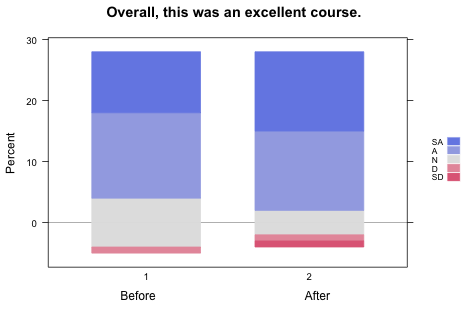
\includegraphics{figures/excellent-course-1.png}

\section{Learning}\label{learning}

\subsection{My interest in the subject has increased because of this
course.}\label{my-interest-in-the-subject-has-increased-because-of-this-course.}

\begin{Shaded}
\begin{Highlighting}[]
\NormalTok{overall.data <-}
\StringTok{  }\NormalTok{te.data }\OperatorTok
\StringTok{  }\KeywordTok{filter}\NormalTok{(Number}\OperatorTok{==}\DecValTok{1632}\NormalTok{) }\OperatorTok
\StringTok{  }\KeywordTok{mutate}\NormalTok{(}\DataTypeTok{Item=}\KeywordTok{as.factor}\NormalTok{(Year))}

\NormalTok{plot.data <-}\StringTok{ }\NormalTok{overall.data[}\DecValTok{7}\OperatorTok{:}\DecValTok{3}\NormalTok{]}
\KeywordTok{rownames}\NormalTok{(plot.data) <-}\StringTok{ }\KeywordTok{c}\NormalTok{(}\StringTok{"Before"}\NormalTok{,}\StringTok{"After"}\NormalTok{)}

\KeywordTok{likert}\NormalTok{(plot.data, }\DataTypeTok{horizontal =} \OtherTok{FALSE}\NormalTok{,}
       \DataTypeTok{main =} \StringTok{"My interest in the subject has increased because of this course."}\NormalTok{,}
       \DataTypeTok{xlab =} \StringTok{"Percent"}\NormalTok{, }\CommentTok{# becomes ylab due to horizontal arg,}
       \DataTypeTok{ylab =} \KeywordTok{c}\NormalTok{(}\StringTok{"Before"}\NormalTok{,}\StringTok{"After"}\NormalTok{),}
       \DataTypeTok{title =} \StringTok{"Overall, this was an excellent course."}\NormalTok{,}
       \DataTypeTok{auto.key =} \KeywordTok{list}\NormalTok{(}\DataTypeTok{space =} \StringTok{"right"}\NormalTok{, }\DataTypeTok{columns =} \DecValTok{1}\NormalTok{,}
                     \DataTypeTok{reverse =} \OtherTok{TRUE}\NormalTok{))}
\end{Highlighting}
\end{Shaded}

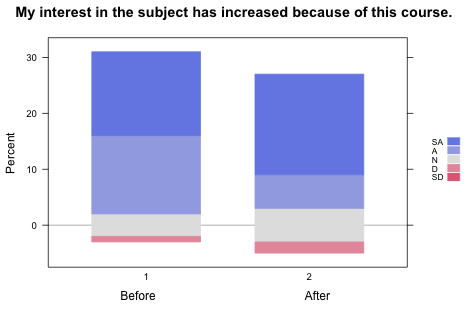
\includegraphics{figures/increased-interest-1.png}

\subsection{I learned a great deal from this
course.}\label{i-learned-a-great-deal-from-this-course.}

\begin{Shaded}
\begin{Highlighting}[]
\NormalTok{overall.data <-}
\StringTok{  }\NormalTok{te.data }\OperatorTok
\StringTok{  }\KeywordTok{filter}\NormalTok{(Number}\OperatorTok{==}\DecValTok{3}\NormalTok{) }\OperatorTok
\StringTok{  }\KeywordTok{mutate}\NormalTok{(}\DataTypeTok{Item=}\KeywordTok{as.factor}\NormalTok{(Year))}

\NormalTok{plot.data <-}\StringTok{ }\NormalTok{overall.data[}\DecValTok{7}\OperatorTok{:}\DecValTok{3}\NormalTok{]}
\KeywordTok{rownames}\NormalTok{(plot.data) <-}\StringTok{ }\KeywordTok{c}\NormalTok{(}\StringTok{"Before"}\NormalTok{,}\StringTok{"After"}\NormalTok{)}

\KeywordTok{likert}\NormalTok{(plot.data, }\DataTypeTok{horizontal =} \OtherTok{FALSE}\NormalTok{,}
       \DataTypeTok{main =} \StringTok{"I learned a great deal from this course.."}\NormalTok{,}
       \DataTypeTok{xlab =} \StringTok{"Percent"}\NormalTok{, }\CommentTok{# becomes ylab due to horizontal arg,}
       \DataTypeTok{ylab =} \KeywordTok{c}\NormalTok{(}\StringTok{"Before"}\NormalTok{,}\StringTok{"After"}\NormalTok{),}
       \DataTypeTok{title =} \StringTok{"Overall, this was an excellent course."}\NormalTok{,}
       \DataTypeTok{auto.key =} \KeywordTok{list}\NormalTok{(}\DataTypeTok{space =} \StringTok{"right"}\NormalTok{, }\DataTypeTok{columns =} \DecValTok{1}\NormalTok{,}
                     \DataTypeTok{reverse =} \OtherTok{TRUE}\NormalTok{))}
\end{Highlighting}
\end{Shaded}

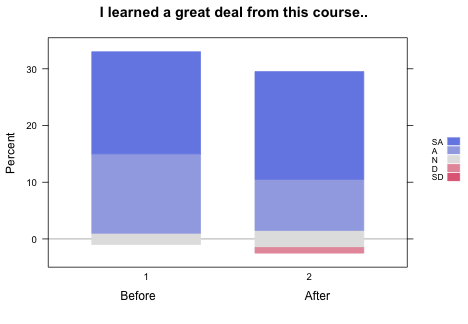
\includegraphics{figures/learned-a-great-deal-1.png}

\subsection{This course advanced my understanding of the subject
matter.}\label{this-course-advanced-my-understanding-of-the-subject-matter.}

\begin{Shaded}
\begin{Highlighting}[]
\NormalTok{overall.data <-}
\StringTok{  }\NormalTok{te.data }\OperatorTok
\StringTok{  }\KeywordTok{filter}\NormalTok{(Number}\OperatorTok{==}\DecValTok{1631}\NormalTok{) }\OperatorTok
\StringTok{  }\KeywordTok{mutate}\NormalTok{(}\DataTypeTok{Item=}\KeywordTok{as.factor}\NormalTok{(Year))}

\NormalTok{plot.data <-}\StringTok{ }\NormalTok{overall.data[}\DecValTok{7}\OperatorTok{:}\DecValTok{3}\NormalTok{]}
\KeywordTok{rownames}\NormalTok{(plot.data) <-}\StringTok{ }\KeywordTok{c}\NormalTok{(}\StringTok{"Before"}\NormalTok{,}\StringTok{"After"}\NormalTok{)}

\KeywordTok{likert}\NormalTok{(plot.data, }\DataTypeTok{horizontal =} \OtherTok{FALSE}\NormalTok{,}
       \DataTypeTok{main =} \StringTok{"This course advanced my understanding of the subject matter."}\NormalTok{,}
       \DataTypeTok{xlab =} \StringTok{"Percent"}\NormalTok{, }\CommentTok{# becomes ylab due to horizontal arg,}
       \DataTypeTok{ylab =} \KeywordTok{c}\NormalTok{(}\StringTok{"Before"}\NormalTok{,}\StringTok{"After"}\NormalTok{),}
       \DataTypeTok{title =} \StringTok{"Overall, this was an excellent course."}\NormalTok{,}
       \DataTypeTok{auto.key =} \KeywordTok{list}\NormalTok{(}\DataTypeTok{space =} \StringTok{"right"}\NormalTok{, }\DataTypeTok{columns =} \DecValTok{1}\NormalTok{,}
                     \DataTypeTok{reverse =} \OtherTok{TRUE}\NormalTok{))}
\end{Highlighting}
\end{Shaded}

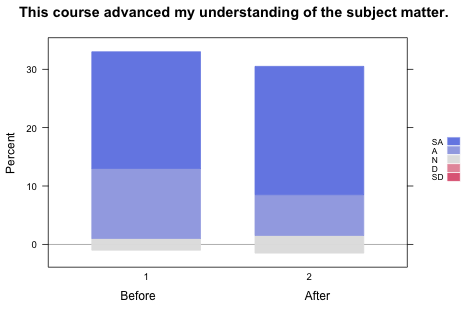
\includegraphics{figures/advanced-understanding-1.png}

\subsection{I learned a great deal from this
course.}\label{i-learned-a-great-deal-from-this-course.-1}

\begin{Shaded}
\begin{Highlighting}[]
\NormalTok{overall.data <-}
\StringTok{  }\NormalTok{te.data }\OperatorTok
\StringTok{  }\KeywordTok{filter}\NormalTok{(Number}\OperatorTok{==}\DecValTok{3}\NormalTok{) }\OperatorTok
\StringTok{  }\KeywordTok{mutate}\NormalTok{(}\DataTypeTok{Item=}\KeywordTok{as.factor}\NormalTok{(Year))}

\NormalTok{plot.data <-}\StringTok{ }\NormalTok{overall.data[}\DecValTok{7}\OperatorTok{:}\DecValTok{3}\NormalTok{]}
\KeywordTok{rownames}\NormalTok{(plot.data) <-}\StringTok{ }\KeywordTok{c}\NormalTok{(}\StringTok{"Before"}\NormalTok{,}\StringTok{"After"}\NormalTok{)}

\KeywordTok{likert}\NormalTok{(plot.data, }\DataTypeTok{horizontal =} \OtherTok{FALSE}\NormalTok{,}
       \DataTypeTok{main =} \StringTok{"I learned a great deal from this course."}\NormalTok{,}
       \DataTypeTok{xlab =} \StringTok{"Percent"}\NormalTok{, }\CommentTok{# becomes ylab due to horizontal arg,}
       \DataTypeTok{ylab =} \KeywordTok{c}\NormalTok{(}\StringTok{"Before"}\NormalTok{,}\StringTok{"After"}\NormalTok{),}
       \DataTypeTok{auto.key =} \KeywordTok{list}\NormalTok{(}\DataTypeTok{space =} \StringTok{"right"}\NormalTok{, }\DataTypeTok{columns =} \DecValTok{1}\NormalTok{,}
                     \DataTypeTok{reverse =} \OtherTok{TRUE}\NormalTok{))}
\end{Highlighting}
\end{Shaded}

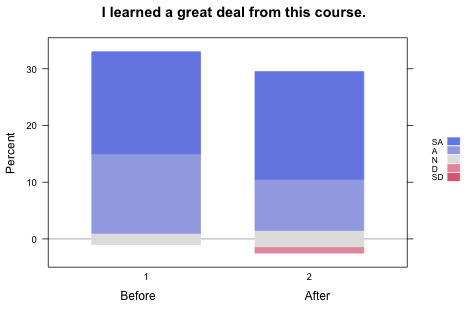
\includegraphics{figures/learned-great-deal-1.png}

\section{Fairness in Grading}\label{fairness-in-grading}

\subsection{The grades in this course were fairly
determined.}\label{the-grades-in-this-course-were-fairly-determined.}

\begin{Shaded}
\begin{Highlighting}[]
\NormalTok{overall.data <-}
\StringTok{  }\NormalTok{te.data }\OperatorTok
\StringTok{  }\KeywordTok{filter}\NormalTok{(Number}\OperatorTok{==}\DecValTok{894}\NormalTok{) }\OperatorTok
\StringTok{  }\KeywordTok{mutate}\NormalTok{(}\DataTypeTok{Item=}\KeywordTok{as.factor}\NormalTok{(Year))}

\NormalTok{plot.data <-}\StringTok{ }\NormalTok{overall.data[}\DecValTok{7}\OperatorTok{:}\DecValTok{3}\NormalTok{]}
\KeywordTok{rownames}\NormalTok{(plot.data) <-}\StringTok{ }\KeywordTok{c}\NormalTok{(}\StringTok{"Before"}\NormalTok{,}\StringTok{"After"}\NormalTok{)}

\KeywordTok{likert}\NormalTok{(plot.data, }\DataTypeTok{horizontal =} \OtherTok{FALSE}\NormalTok{,}
       \DataTypeTok{main =} \StringTok{"The grades in this course were fairly determined."}\NormalTok{, }\CommentTok{# or give "title",}
       \DataTypeTok{xlab =} \StringTok{"Percent"}\NormalTok{, }\CommentTok{# becomes ylab due to horizontal arg,}
       \DataTypeTok{ylab =} \KeywordTok{c}\NormalTok{(}\StringTok{"Before"}\NormalTok{,}\StringTok{"After"}\NormalTok{),}
       \DataTypeTok{title =} \StringTok{"Overall, this was an excellent course."}\NormalTok{,}
       \DataTypeTok{auto.key =} \KeywordTok{list}\NormalTok{(}\DataTypeTok{space =} \StringTok{"right"}\NormalTok{, }\DataTypeTok{columns =} \DecValTok{1}\NormalTok{,}
                     \DataTypeTok{reverse =} \OtherTok{TRUE}\NormalTok{))}
\end{Highlighting}
\end{Shaded}

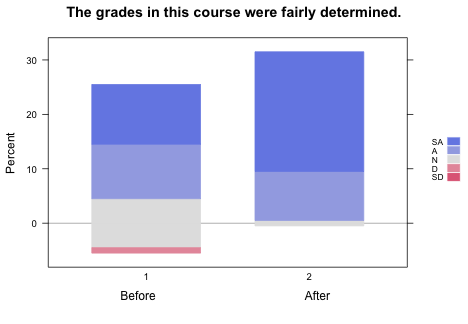
\includegraphics{figures/grades-fairly-determined-1.png}

\subsection{Graded assignments reflected the material
covered}\label{graded-assignments-reflected-the-material-covered}

\begin{Shaded}
\begin{Highlighting}[]
\NormalTok{overall.data <-}
\StringTok{  }\NormalTok{te.data }\OperatorTok
\StringTok{  }\KeywordTok{filter}\NormalTok{(Number}\OperatorTok{==}\DecValTok{893}\NormalTok{) }\OperatorTok
\StringTok{  }\KeywordTok{mutate}\NormalTok{(}\DataTypeTok{Item=}\KeywordTok{as.factor}\NormalTok{(Year))}

\NormalTok{plot.data <-}\StringTok{ }\NormalTok{overall.data[}\DecValTok{7}\OperatorTok{:}\DecValTok{3}\NormalTok{]}
\KeywordTok{rownames}\NormalTok{(plot.data) <-}\StringTok{ }\KeywordTok{c}\NormalTok{(}\StringTok{"Before"}\NormalTok{,}\StringTok{"After"}\NormalTok{)}

\KeywordTok{likert}\NormalTok{(plot.data, }\DataTypeTok{horizontal =} \OtherTok{FALSE}\NormalTok{,}
       \DataTypeTok{main =} \StringTok{"Graded assignments reflected the material covered."}\NormalTok{, }\CommentTok{# or give "title",}
       \DataTypeTok{xlab =} \StringTok{"Percent"}\NormalTok{, }\CommentTok{# becomes ylab due to horizontal arg,}
       \DataTypeTok{ylab =} \KeywordTok{c}\NormalTok{(}\StringTok{"Before"}\NormalTok{,}\StringTok{"After"}\NormalTok{),}
       \DataTypeTok{title =} \StringTok{"Overall, this was an excellent course."}\NormalTok{,}
       \DataTypeTok{auto.key =} \KeywordTok{list}\NormalTok{(}\DataTypeTok{space =} \StringTok{"right"}\NormalTok{, }\DataTypeTok{columns =} \DecValTok{1}\NormalTok{,}
                     \DataTypeTok{reverse =} \OtherTok{TRUE}\NormalTok{))}
\end{Highlighting}
\end{Shaded}

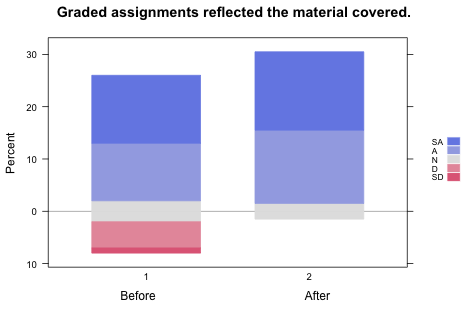
\includegraphics{figures/reflected-material-1.png}

\subsection{Knew what was expected of
me}\label{knew-what-was-expected-of-me}

\begin{Shaded}
\begin{Highlighting}[]
\NormalTok{overall.data <-}
\StringTok{  }\NormalTok{te.data }\OperatorTok
\StringTok{  }\KeywordTok{filter}\NormalTok{(Number}\OperatorTok{==}\DecValTok{1633}\NormalTok{) }\OperatorTok
\StringTok{  }\KeywordTok{mutate}\NormalTok{(}\DataTypeTok{Item=}\KeywordTok{as.factor}\NormalTok{(Year))}

\NormalTok{plot.data <-}\StringTok{ }\NormalTok{overall.data[}\DecValTok{7}\OperatorTok{:}\DecValTok{3}\NormalTok{]}
\KeywordTok{rownames}\NormalTok{(plot.data) <-}\StringTok{ }\KeywordTok{c}\NormalTok{(}\StringTok{"Before"}\NormalTok{,}\StringTok{"After"}\NormalTok{)}

\KeywordTok{likert}\NormalTok{(plot.data, }\DataTypeTok{horizontal =} \OtherTok{FALSE}\NormalTok{,}
       \DataTypeTok{main =} \StringTok{"I knew what was expected of me in this course.."}\NormalTok{, }\CommentTok{# or give "title",}
       \DataTypeTok{xlab =} \StringTok{"Percent"}\NormalTok{, }\CommentTok{# becomes ylab due to horizontal arg,}
       \DataTypeTok{ylab =} \KeywordTok{c}\NormalTok{(}\StringTok{"Before"}\NormalTok{,}\StringTok{"After"}\NormalTok{),}
       \DataTypeTok{title =} \StringTok{"Overall, this was an excellent course."}\NormalTok{,}
       \DataTypeTok{auto.key =} \KeywordTok{list}\NormalTok{(}\DataTypeTok{space =} \StringTok{"right"}\NormalTok{, }\DataTypeTok{columns =} \DecValTok{1}\NormalTok{,}
                     \DataTypeTok{reverse =} \OtherTok{TRUE}\NormalTok{))}
\end{Highlighting}
\end{Shaded}

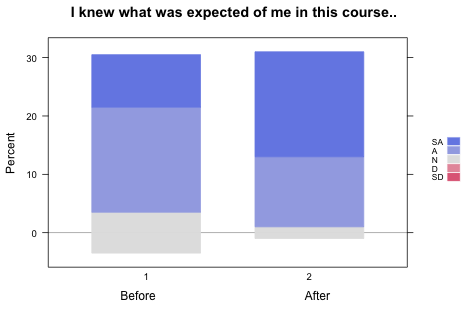
\includegraphics{figures/knew-expectations-1.png}

\section{Workload}\label{workload}

\begin{Shaded}
\begin{Highlighting}[]
\NormalTok{overall.data <-}
\StringTok{  }\NormalTok{te.data }\OperatorTok
\StringTok{  }\KeywordTok{filter}\NormalTok{(Number}\OperatorTok{==}\DecValTok{891}\NormalTok{) }\OperatorTok
\StringTok{  }\KeywordTok{mutate}\NormalTok{(}\DataTypeTok{Item=}\KeywordTok{as.factor}\NormalTok{(Year))}

\NormalTok{plot.data <-}\StringTok{ }\NormalTok{overall.data[}\DecValTok{7}\OperatorTok{:}\DecValTok{3}\NormalTok{]}
\KeywordTok{rownames}\NormalTok{(plot.data) <-}\StringTok{ }\KeywordTok{c}\NormalTok{(}\StringTok{"Before"}\NormalTok{,}\StringTok{"After"}\NormalTok{)}

\KeywordTok{likert}\NormalTok{(plot.data, }\DataTypeTok{horizontal =} \OtherTok{FALSE}\NormalTok{,}
       \DataTypeTok{main =} \StringTok{"As compared with other courses of equal credit, the workload of this course was:"}\NormalTok{, }\CommentTok{# or give "title",}
       \DataTypeTok{xlab =} \StringTok{"Percent"}\NormalTok{, }\CommentTok{# becomes ylab due to horizontal arg,}
       \DataTypeTok{ylab =} \KeywordTok{c}\NormalTok{(}\StringTok{"Before"}\NormalTok{,}\StringTok{"After"}\NormalTok{),}
       \DataTypeTok{title =} \StringTok{"Overall, this was an excellent course."}\NormalTok{,}
       \DataTypeTok{auto.key =} \KeywordTok{list}\NormalTok{(}\DataTypeTok{space =} \StringTok{"right"}\NormalTok{, }\DataTypeTok{columns =} \DecValTok{1}\NormalTok{,}
                     \DataTypeTok{reverse =} \OtherTok{TRUE}\NormalTok{))}
\end{Highlighting}
\end{Shaded}

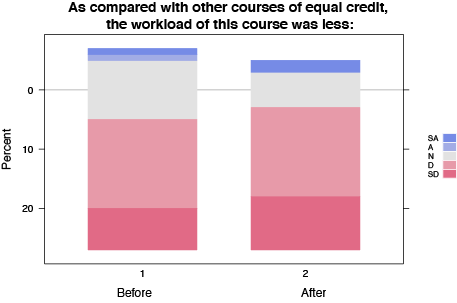
\includegraphics{figures/workload-1.png}


\end{document}
